% Legacy merge file — canonical sources: paper/tables/fig_*.tex

The following figures complement Tables~\ref{tab:S1}--\ref{tab:S5}.
They follow the Capobianco \emph{et al.}~\cite{Capobianco2024electron} observable set at the main-text PBE+D3 level and are \emph{orthogonal} to the $\mathcal{S}$ audit.

\begin{figure}[!ht]
\centering
\IfFileExists{figures/out/figure_s1_pdos_exp7.pdf}{%
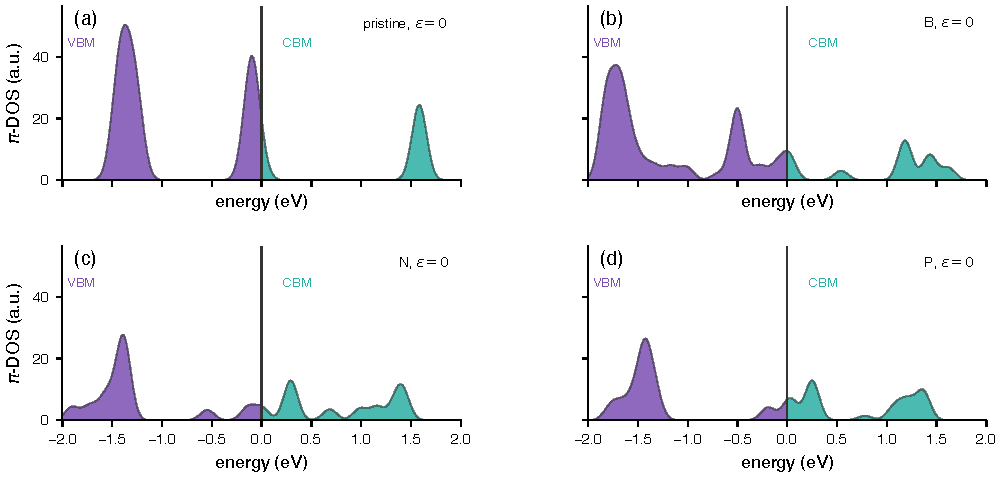
\includegraphics[width=0.88\textwidth]{figures/out/figure_s1_pdos_exp7.pdf}}{%
\fbox{\parbox{0.85\textwidth}{\centering\vspace{2cm}\textbf{PDOS figure not found}\vspace{2cm}}}%
}
\caption{\label{fig:S1}$\pi$-projected density of states ($\pi$-DOS) for pristine and B/N/P-doped tetramers at $\epsilon{=}0$ (PBE+D3).
Panels (a)--(d) share a common vertical scale; energy is relative to the Fermi level at 0~eV (Capobianco color scheme~\cite{Capobianco2024electron}).}
\end{figure}


\begin{figure}[!ht]
\centering
\IfFileExists{figures/out/figure_s2_marcus.pdf}{%
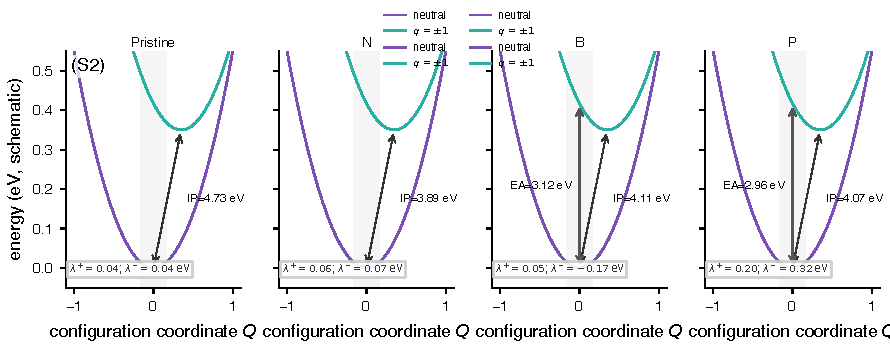
\includegraphics[width=0.88\textwidth]{figures/out/figure_s2_marcus.pdf}}{%
\fbox{\parbox{0.85\textwidth}{\centering\vspace{2cm}\textbf{Marcus figure not found}\vspace{2cm}}}%
}
\caption{\label{fig:S2}Marcus reorganization energies (12/12 charged-state geometry optimizations; eight vertical single-points at the neutral geometry).
Pristine $\lambda^{\pm}{=}0.041$/0.042~eV; N $\lambda^{+}{=}0.058$/ $\lambda^{-}{=}0.065$~eV; B $\lambda^{+}{=}0.051$~eV; P $\lambda^{+}{=}0.200$/ $\lambda^{-}{=}0.315$~eV.
The electron-channel reorganization energy $\lambda^{-}$ for B doping is unphysical under the fixed neutral-geometry vertical protocol and is excluded (Limitations).}
\end{figure}


\begin{figure}[!ht]
\centering
\IfFileExists{figures/out/figure_s3_j_exp4.pdf}{%
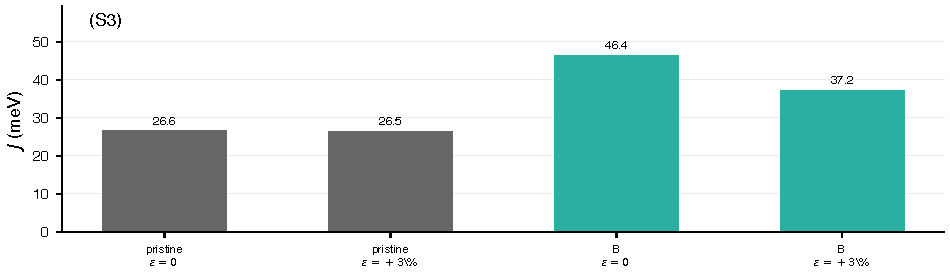
\includegraphics[width=0.88\textwidth]{figures/out/figure_s3_j_exp4.pdf}}{%
\fbox{\parbox{0.85\textwidth}{\centering\vspace{1.5cm}\textbf{IPR/$J$ figure not found}\vspace{1.5cm}}}%
}
\caption{\label{fig:S3}Nearest-neighbor electronic coupling $J$ on the tetramer dimer grid (pristine and B-doped cells at $\epsilon{=}0$ and $+3$\%; PBE+D3).}
\end{figure}



On the tetramer dimer grid, B substitution at $\epsilon{=}0$ delocalizes the charged-state orbital (IPR $75.0\rightarrow 24.6$) while raising $J$ from $26.6$ to $46.4$~meV; coupled B @ $+3$\% gives $J=37.2$~meV and IPR $23.1$.
The criterion $J>\lambda/2$ for polaron hopping dominance~\cite{Capobianco2024electron} is \emph{not} met at PBE+D3 ($J<\lambda/2$), so a polaron transition is not confirmed on this grid.

